\newpage
\section{Network and Security}
To provide their customers security regarding their information, Smoking Games maintain their own in-house IT-system and file storage. This also gives the employees easy access to customer information with respect to the C.I.A. principles (confidentiality, integrity, availability).
\subsection{Network}
Smoking Games host their own Web services. Maintenance of these services and the rest of the network is the responsibility of Smoking Games' own IT department.\\
The company network is divided in, roughly speaking, three parts: the public network (DMZ), the internal network and the wireless network. An overview of the network topology is shown in figure \ref{fig:net_top}.\\
All connections between the outside and the internal network or the DMZ are being filtered by the external router which has a firewall included. The DMZ (demilitarized zone) contains public services such as a Web server or a VPN server (used for e.g. consulting purposes). Access to these services is restricted and handled by, as mentioned, the external router, which is configured to route packets between the outside and the DMZ differently than between the outside and the internal network. Additionally and IDS/IPS (incident detection/incident prevention system) is placed between the public network and the external router.\\
In case of a compromised external router all connectios between the outside and the internal network are being protected by an IDS/IPS and an internal router, which has additional filer lists implemented.\\
All information and data about customers or other business aspects are stored on the database server and file storage, respectively. Access to this data is handled by a router with a strictly configured firewall, so to avoid unauthorized access.\\
The rest of the internal network consists of work machines and a print server and printer.\\
A wireless network is also being provided, but it is not connected to the other network to avoid that information about customers or business projects is being stored on personal mobile devices.
\begin{figure}[h]\centering
	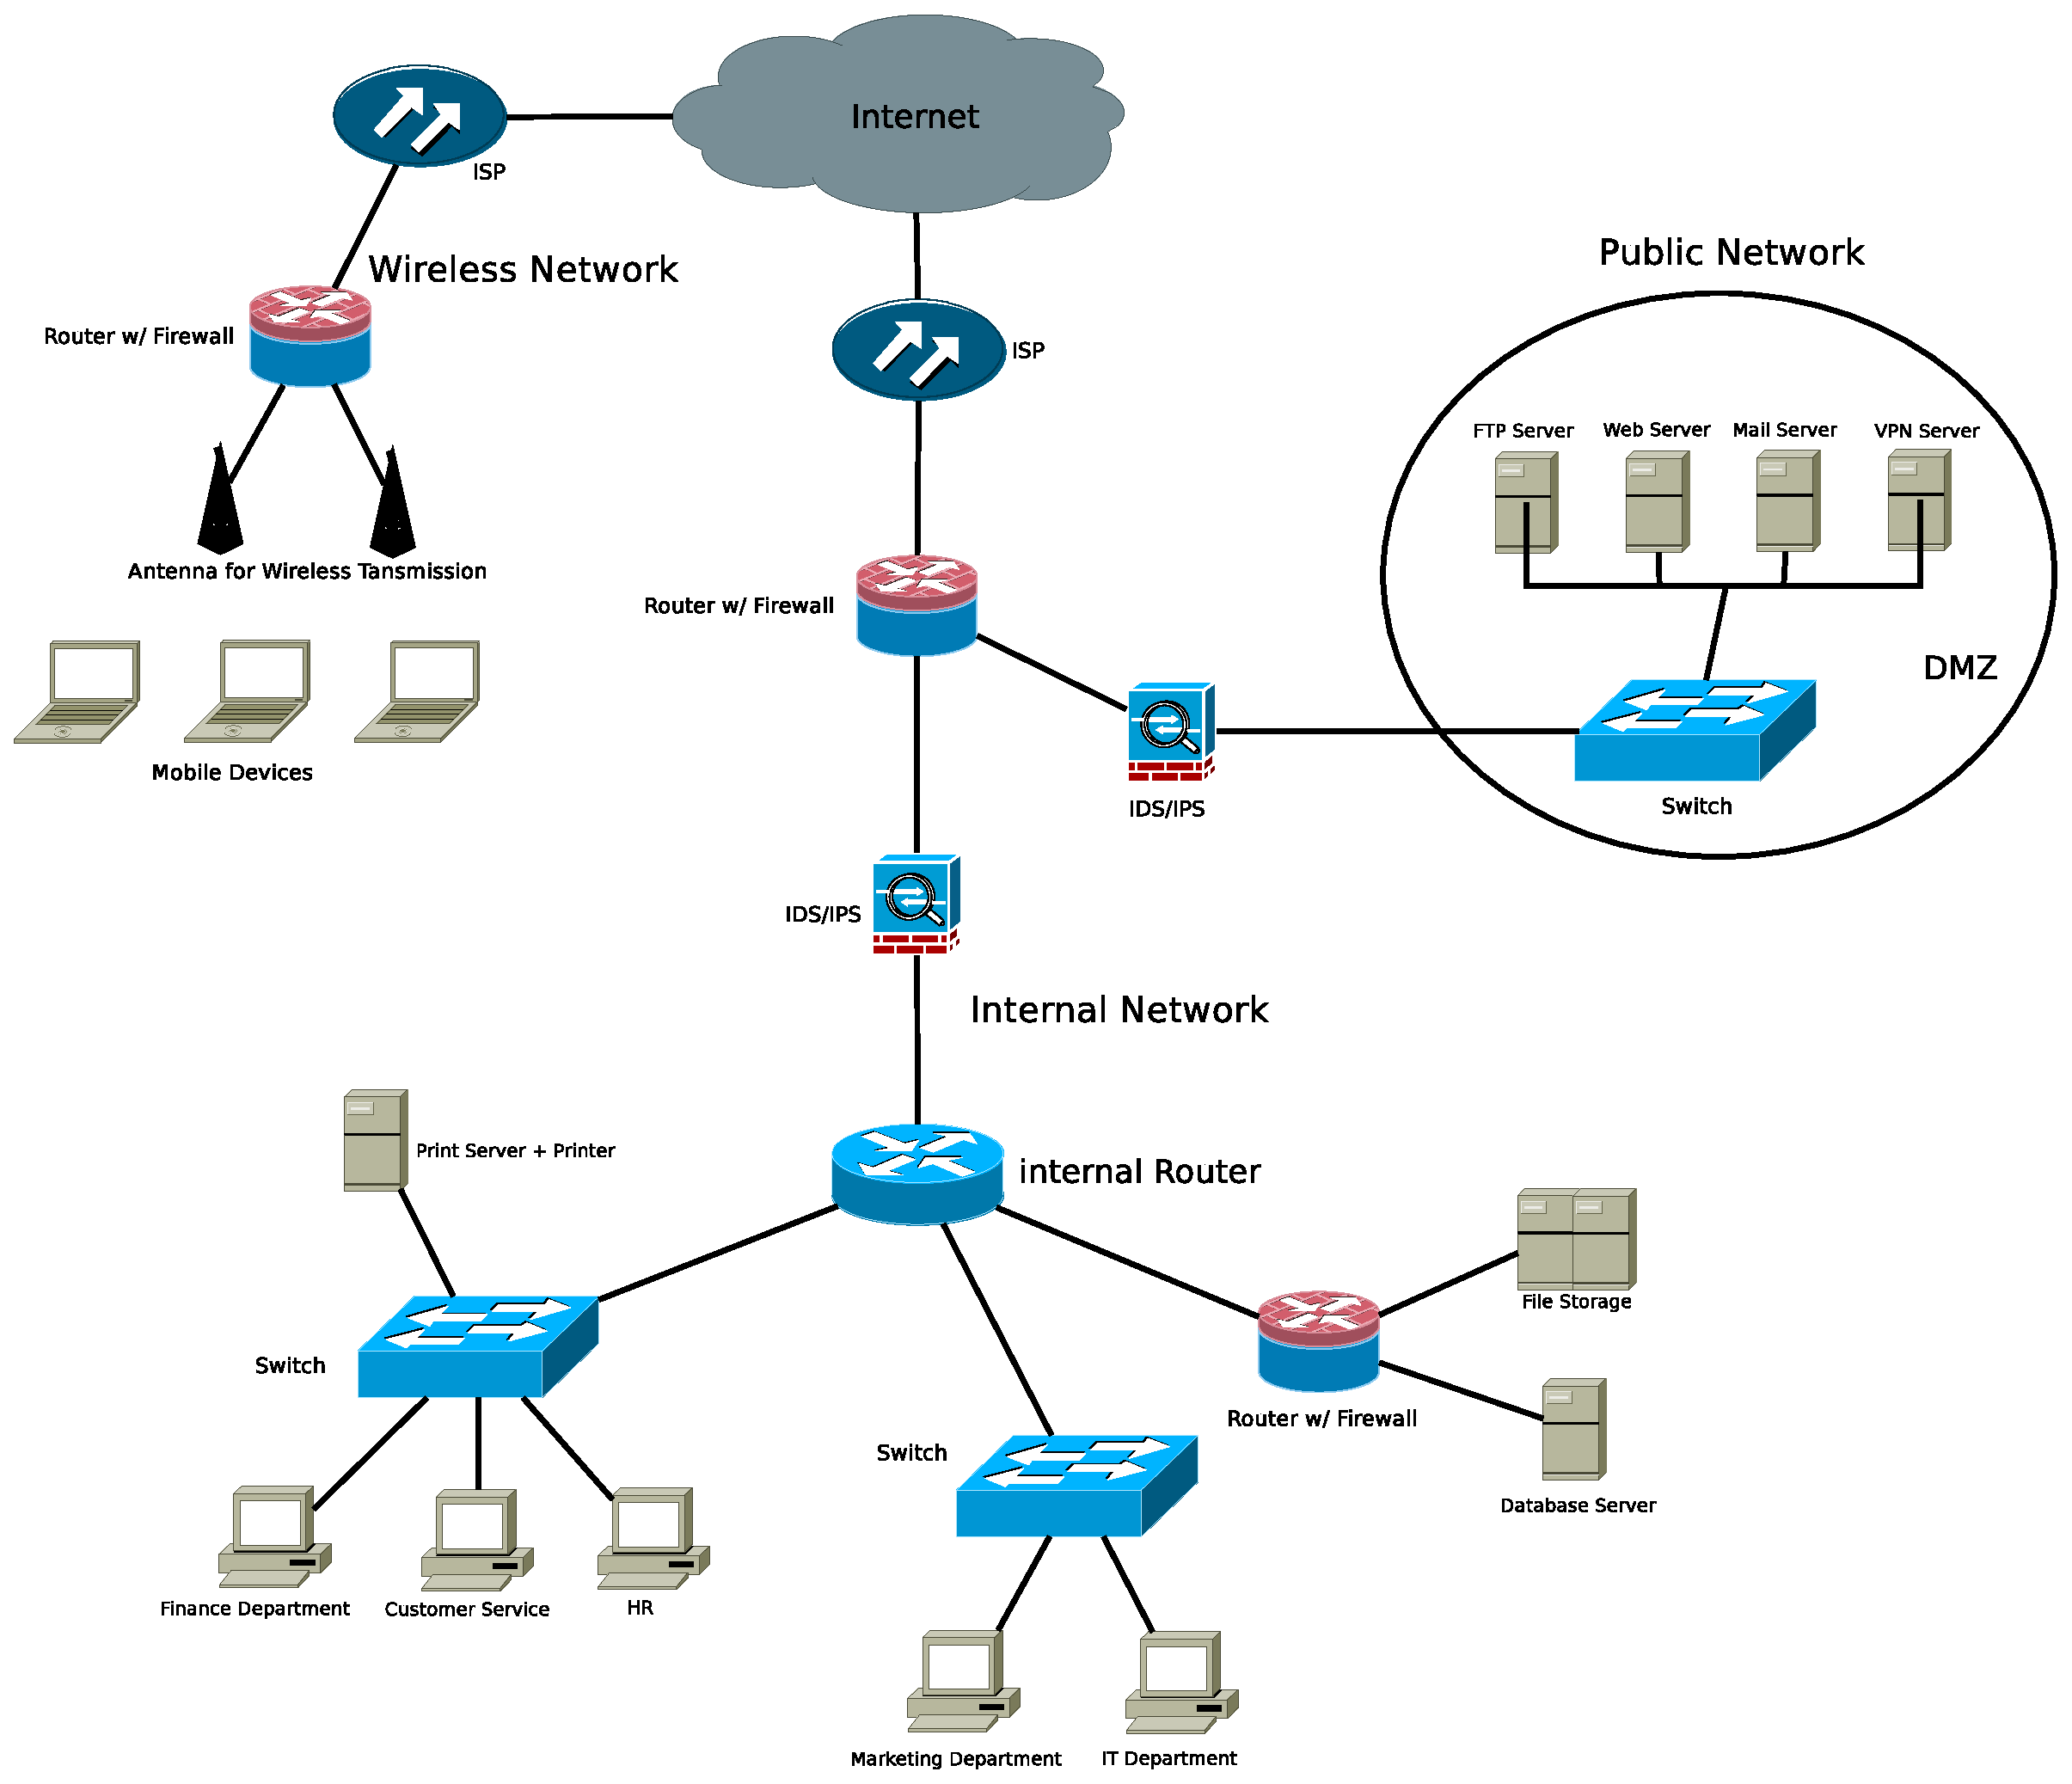
\includegraphics[scale=.3]{pictures/network_topology.eps}
	\caption{Network Topology}
	\label{fig:net_top}
\end{figure}
\subsection{Rules and Regulation}
As BYOD (bring your own device) is becoming more and more a security risk for companies, Smoking Games have strict policies for personal mobile devices. They are only allowed to use in the wireless area and (of course) outside the company network. Also, no information regarding the customers or business projects is allowed to keep or use on the devices. Flash drives provided by Smoking Games are encrypted and have an installed anti-spyware protable scanner to keep them free of malware. They are allowed to use inside the companies network, but not in the wireless area or outside of the building. The same applies for other mobile devices provided by Smoking Games.\\
All employees are required to properly secure their work equipment as a part of the employee contract they have signed with the company. In return the company promises to give adequate education on how to secure their equipment. This kind of security measures includes anti-virus,
secure communication, physical security, clear-desk policy and other relevant topics. Also, the security team has to make sure, that on every machine the latest security updates are installed.\\
Smoking Games have an incremental daily backup strategy and a complete back-up each Friday night. These back-ups are stored both on site and off site. The off site storage facility is a third party service provider, which complies with the same policies and legislative demands as Smoking Games.\\